\chapter{Hipótesis y objetivos} % Main chapter title
\label{sec:Hipotesis} % For referencing the chapter elsewhere, use

\section{Pregunta de Investigación}
\label{sec:pregunta}

Identificado el vacío en la literatura respecto a la ausencia de mecanismos formales de revisión histórica por parte de los fiscalizadores en entornos de aprendizaje social, y considerando la interacción entre la memoria institucional del ente fiscalizador, la memoria social de los contribuyentes y la estrategia de fiscalización empleada, la presente investigación plantea la siguiente pregunta central:

¿De qué manera la inclusión de una profundidad variable de memoria institucional (capacidad de realizar auditorías retrospectivas sujetas a ruido de detección) por parte del ente fiscalizador interactúa con la memoria social de los contribuyentes y con la estrategia de fiscalización empleada para afectar las tasas a largo plazo de cumplimiento tributario y evasión fiscal en un Modelo Basado en Agentes?

A través de la resolución de esta interrogante, se busca entregar herramientas concretas para la calibración óptima de políticas públicas de fiscalización, identificando qué estrategia es preferible en cada contexto y maximizando el impacto de cada auditoría en ecosistemas sociales altamente adaptativos.

\section{Hipótesis}
\label{sec:hipotesis}

\subsection{Hipótesis principal}
\label{sec:h1}

\textbf{H1.} La inclusión de memoria institucional por parte del ente fiscalizador reduce significativamente las tasas de evasión fiscal a largo plazo en el ABM, y este efecto se modula simultáneamente por la extensión de la memoria social de los contribuyentes y por la estrategia de fiscalización empleada.

\subsection{Hipótesis secundarias}
\label{sec:h2-secundarias}

\textbf{H2.} Aumentar la profundidad de la memoria institucional reduce la evasión, pero la magnitud del efecto decrece a medida que aumenta el ruido de detección: a mayor degradación de la información histórica, menor el retorno disuasivo marginal de prolongar la ventana retrospectiva.

\textbf{H3.} El efecto de la memoria institucional sobre el cumplimiento depende del nivel de memoria social: con memoria social corta, una memoria institucional profunda refuerza el efecto disuasivo de las estrategias focalizadas; con memoria social larga, el efecto adicional de la memoria institucional se atenúa porque los contribuyentes ya acumulan información vecinal estabilizadora.

\textbf{H4.} Bajo memorias institucionales profundas, la estrategia de focalización estratégica supera a la aleatoria; bajo memorias institucionales superficiales, la auditoría aleatoria alcanza desempeño marginalmente equivalente, reproduciendo el patrón que \textcite{canessa2025tax} observó al variar la memoria social. La focalización por nivel de ingreso rinde consistentemente por debajo de ambas.

\textbf{H5.} Bajo una profundidad institucional elevada, la auditoría aleatoria rinde peor que bajo profundidad institucional nula, porque extender la ventana retrospectiva redistribuye la misma fuerza de auditoría sobre más períodos por agente, reduciendo la cobertura horizontal de contribuyentes efectivamente auditados y, con ello, la probabilidad agregada de detección.

\section{Objetivos}
\label{sec:objetivos}

\subsection{Objetivo general}
\label{sec:obj-general}

Desarrollar y evaluar un Modelo Basado en Agentes que extienda el modelo de \textcite{canessa2025tax} incorporando memoria institucional parametrizable (profundidad retrospectiva y ruido de detección), para caracterizar la interacción tripartita entre memoria institucional, memoria social y estrategia de fiscalización sobre el cumplimiento tributario a largo plazo.

\subsection{Objetivos específicos}
\label{sec:obj-especificos}

\begin{enumerate}
  \item Extender el ABM de Canessa incorporando un submodelo de auditoría retrospectiva con parámetros de profundidad $k$ y ruido de detección, conservando intacta la dinámica de aprendizaje social del modelo base.
  \item Ejecutar un diseño factorial que combine niveles de memoria institucional, memoria social y estrategia de fiscalización, manteniendo constantes los demás parámetros del modelo base.
  \item Analizar estadísticamente las interacciones entre las tres variables independientes sobre las métricas de cumplimiento, aversión al riesgo y detección de fraudes.
  \item Formular recomendaciones de política pública que identifiquen qué estrategia de fiscalización es preferible bajo cada configuración de memoria institucional y memoria social, maximizando el impacto disuasivo y recaudatorio con el menor costo administrativo posible.
\end{enumerate}

\section{Propuesta metodológica}
\label{sec:propuesta}

La presente investigación se desarrolla sobre el Modelo Basado en Agentes (ABM) de cumplimiento tributario de \textcite{canessa2025tax}, que simula una sociedad heterogénea de contribuyentes que aprenden estrategias de evasión mediante aprendizaje por refuerzo en una vecindad Moore, e interactúan con un ente fiscalizador que despliega distintas estrategias de auditoría. La estructura del modelo ha sido documentada formalmente mediante el protocolo vODD (Visual Overview, Design concepts and Details), una herramienta de especificación visual diseñada para facilitar la comprensión, replicación y extensión de modelos basados en agentes. El diagrama visual correspondiente se presenta en la Figura~\ref{fig:odd-visual}.

\begin{figure}[ht]
	\centering
	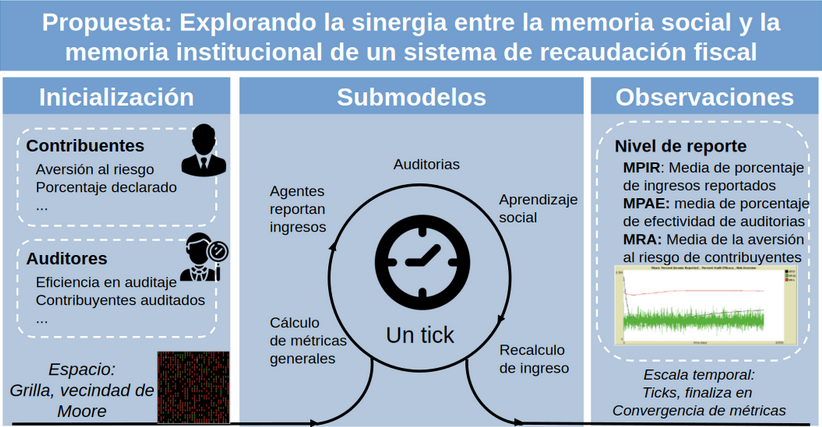
\includegraphics[width=0.95\columnwidth]{Figures/ODD_Visual_modeloNuevo.png}
	\caption{Diagrama visual vODD del modelo ABM de cumplimiento tributario extendido con memoria institucional.}
	\label{fig:odd-visual}
\end{figure}

El modelo original de Canessa contempla un submodelo de auditorías en el cual el fiscalizador evalúa exclusivamente el período corriente de declaración de cada contribuyente, es decir, opera sin memoria retrospectiva. Esta investigación extiende dicho submodelo introduciendo el concepto de \textit{ventana de auditoría}, que permite al auditor inspeccionar entre 1 y 15 períodos fiscales anteriores al actual. La profundidad de esta ventana constituye la variable independiente denominada \textit{Memoria Institucional}, la cual se combina con un parámetro de degradación progresiva (\textit{Ruido de Detección}) que modela la pérdida natural de precisión conforme los registros históricos se alejan del presente.

El diseño experimental combina tres factores: la memoria institucional (con su profundidad y ruido), la memoria social de los contribuyentes (factor \textit{period-frauds} del modelo base) y la estrategia de fiscalización (aleatoria, focalización por nivel de ingreso o focalización estratégica por puntaje de riesgo). El submodelo extendido conserva intacta la dinámica de aprendizaje social entre contribuyentes y las reglas de interacción vecinal del modelo base, aislando así el efecto causal de la memoria institucional sobre las tasas de cumplimiento tributario a largo plazo.

\section{Variables y operacionalización}
\label{sec:variables}

\subsection{Variables independientes}
\label{sec:vi}

El diseño experimental manipula tres variables independientes:

\begin{itemize}
  \item \textbf{Profundidad de la memoria institucional} ($k$): número de períodos fiscales anteriores que el auditor puede revisar. Se adopta el dominio experimental $k \in \{1, 5, 10, 15\}$, cubriendo desde un único período retrospectivo hasta una ventana extensa plausible en la práctica regulatoria.
  \item \textbf{Ruido de detección}: probabilidad de que la auditoría de un período lejano no detecte correctamente una subdeclaración previa \parencite{debacker2018once}. Se adoptan los niveles $\{0;\, 0{,}1;\, 0{,}3;\, 0{,}5\}$, desde detección perfecta hasta una degradación elevada.
  \item \textbf{Memoria social} (PF, \textit{period-frauds}): número de períodos hacia atrás que cada agente observa a sus vecinos en la vecindad Moore. Se replican los niveles del modelo de Canessa, $PF \in \{1, 5\}$, que se asocian respectivamente a memoria social corta y larga.
  \item \textbf{Estrategia de fiscalización}: aleatoria, focalización por nivel de ingreso o focalización estratégica por puntaje de riesgo, conforme a las tres estrategias contrastadas por \textcite{canessa2025tax}.
\end{itemize}

\subsection{Variables dependientes}
\label{sec:vd}

Las variables de respuesta corresponden a las métricas de estado estacionario del modelo:

\begin{itemize}
  \item \textbf{PIAR} (\textit{Percent of Income Actually Reported}): porcentaje medio de ingreso efectivamente reportado por los contribuyentes, principal indicador de cumplimiento tributario.
  \item \textbf{MRA} (\textit{Mean Risk Aversion}): nivel medio de aversión al riesgo,indicador del proceso de aprendizaje adaptativo.
  \item \textbf{PDF} (\textit{Percent of Detected Frauds}): porcentaje de fraudes detectados, calculado como el cociente entre el número acumulado de fraudes detectados y el número acumulado de fraudes cometidos.
\end{itemize}

\subsection{Dominio experimental}
\label{sec:dominio}

Las métricas se medirán en el régimen de estado pseudo-estacionario del modelo, entre los pasos de simulación $25.000$ y $30.000$, conforme al protocolo de Canessa, que evidencia estabilización a partir del paso $10.000$. Cada combinación de factores se ejecutará múltiples veces para asegurar potencia estadística adecuada, manteniendo constantes los demás parámetros del modelo base (número de contribuyentes, tasa de auditoría, tasa de impuestos, penalidad, tasa de aprendizaje y nivel inicial de aversión al riesgo).